\label{ch:related-works}

Many works have already been done for the visualization of spatio-temporal data that can inspire further improvements and adaptations.
%
We now present an overview of spatio-temporal visualization, starting from conventional methods commonly used and after presenting recent works in the area of spatio-temporal visualization.

\section{Spatio-temporal visualization}

Map visualization has been used for more than centuries and has an extensive search done.
%
Recently, with the increase of spatio-temporal data, the most used methods for visualization uses the techniques from cartography to represent spatial information and the dynamic aspect of computer-based visualizations to represent time: interactivity and animations. 
%
To present an overview of the spatio-temporal visualizations already made, we will talk about widely used techniques and recent works that inspire and relate to Events-Vis.

\subsection{Space-time cube}

The Space-Time Cube, as the name says, is a plot created with the use of a three-dimensional cube such that the base represents the 2D space and the height represents the time dimension~\cite{bach2017descriptive}.
%
With that formulation, the STC is a very general method and supports different graphic primitives to represent different types of data and different types of attributes, such as trajectories, events, with categorical or numerical attributes.
%

Figure~\ref{fig:space-time-cube-reference} is shown the use of a STC for a trajectory, on the base of the cube is drawn a map of the city that the data is from, and a black line is marked linking the points of the personal travel during the day, as the black line increases in the height, it indicates the passing time. On the visualization are some marks to increase the interpretability, and for example, it is possible to check that the person left the house at 05:10 and returned at 19:55.

\begin{figure}
    \centering
    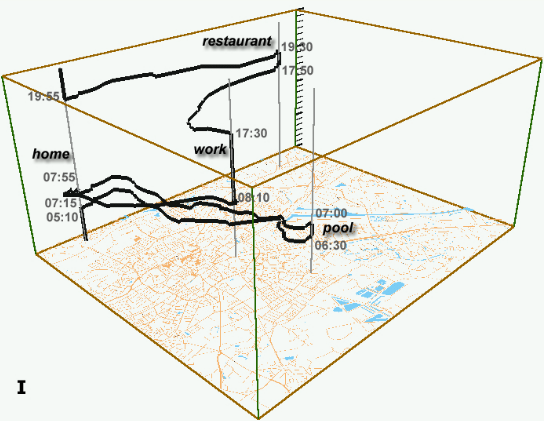
\includegraphics[width = 0.7\textwidth]{src/imgs/space-time-cube-reference.png}
    \caption{Source: \cite{Kraak2003Space}. Space-Time Cube visualization of a trajectory of a routine day of a person in a city.}
    \label{fig:space-time-cube-reference}
\end{figure}
%
Many visualizations use the STC linked to other views to permit better analyses of the data with other attributes than the spatio-temporal information.
%
However, as the cube is a 3D object represented in a 2D screen of a computer, it is necessary a projection that can lead to bad positioning of the graphic primitives, causing cluttering and distortion of space and time~\cite{andrienko2013visual}.
%
In the example in Fig.~\ref{fig:space-time-cube-reference}, it is not totally possible to compare the distance between \textit{pool} and \textit{work}, and the distance between \textit{work} and \textit{restaurant} due to the projection of the 3D cube.

\subsection{Small-multiples}

Small-multiples is a visualization method that uses sequential map plots to represent the time evolution of the data, the total time interval is divided into smaller periods and the data from each period is plotted in a separated map.
%
This method permits the flexibility to use any map visualization that do not consider the time, and just create it for different fixed time intervals.
%
In Figure~\ref{fig:small-multiples-reference} is presented a small multiple visualization of the progress of approved land for harvesting in the Hood Canal. 
%
Each of the individual eleven maps represents a year of the data and uses coloring in each to mark the approved areas.

\begin{figure}
    \centering
    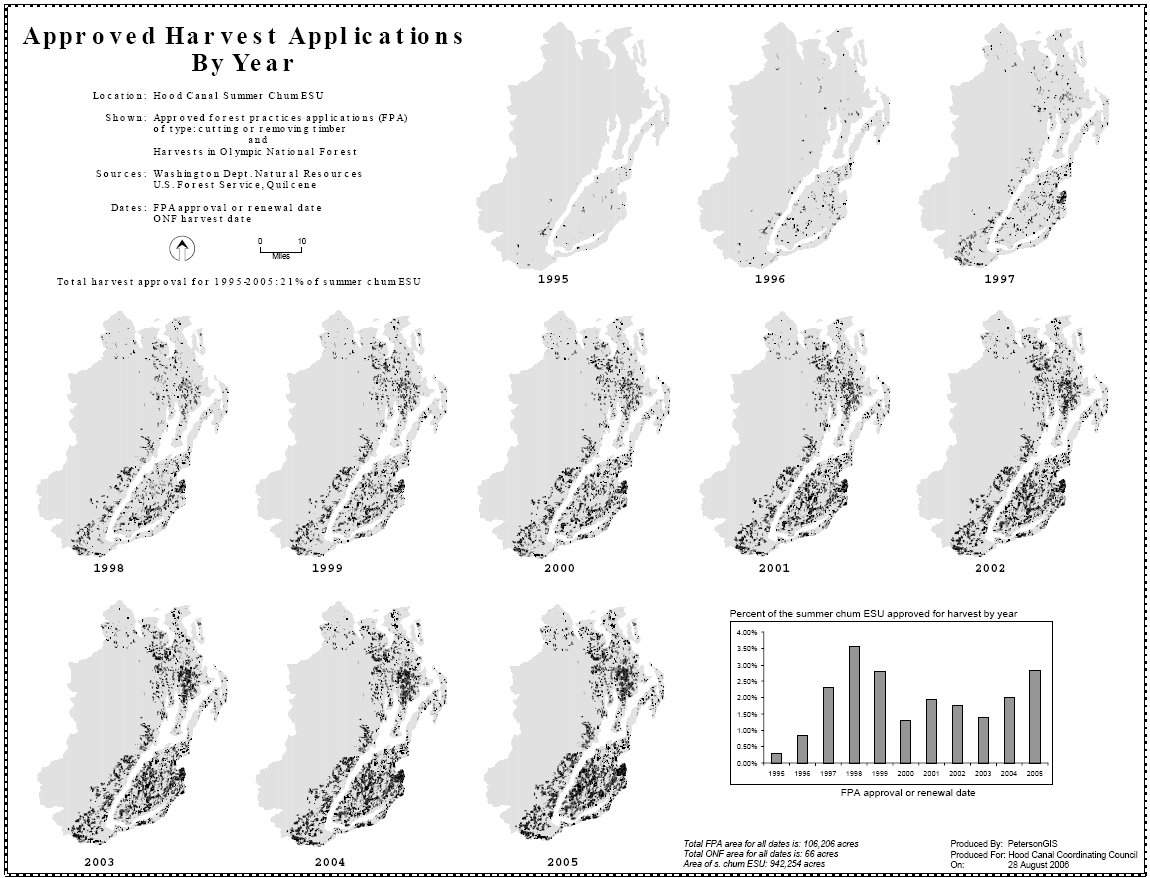
\includegraphics[width = \textwidth]{src/imgs/small-multiples-reference.jpg}
    \caption{Source: \cite{peterson2011small}. A yearly time-series of the approved lands for harvesting in on Hood Canal plotted with a small multiples visualization.}
    \label{fig:small-multiples-reference}
\end{figure}

However, a limitation to the method is the number of views that can be represented on the screen, as the number can not get big, and that it is not simple to identify the best detail to discretize time and generate the multiple views~\cite{Andrienko2003exploratory}.
%
As shown in the example, the  maps take a big screen size and are limited to an interval of eleven years.

\subsection{Animations}

Animations can be used in any form of visualization, it permits to update the figure with new information and can lead the attention of the viewer.
%
On spatio-temporal data, basic map plots are created to represent the 2D space and the time is represented by the physical time, i.e., the pass of the time in the data is represented with the pass of the real-time.
%
To increase the quality of the visualization, the user can select intervals where they want to visualize the animation, jumps between timestamps, control the velocity.
%

However, even with this flexibility of control, animations visualization suffers from a cognitive limitation.
%
To compare data from different timestamps, the user needs to memorize the figure as it is not possible to visualize them simultaneously, and as already known, the human brain can keep track of only a small number of changing objects~\cite{Harrower:2007:Cognitive}. 
%
\subsection{Recent methods}
%
With most visualization tools proposed for spatio-temporal data using linked views and interactivity, some recent methods have been using static 2D plots to represent an overview of the data.
%
The idea is to represent the space as a function of time, and as usual, the time is represented in the horizontal.
%
With that, the 2D space is represented in a 1D vertical axis and a projection method is necessary to make this space transformation.

With minor changes according to the objective, some of the examples of this method are: \cite{Buchmuller:2018:MVCTST}, \cite{spatialrugs}, \cite{wulms2021stable} and \cite{1dordering}.

\begin{figure}
    \centering
    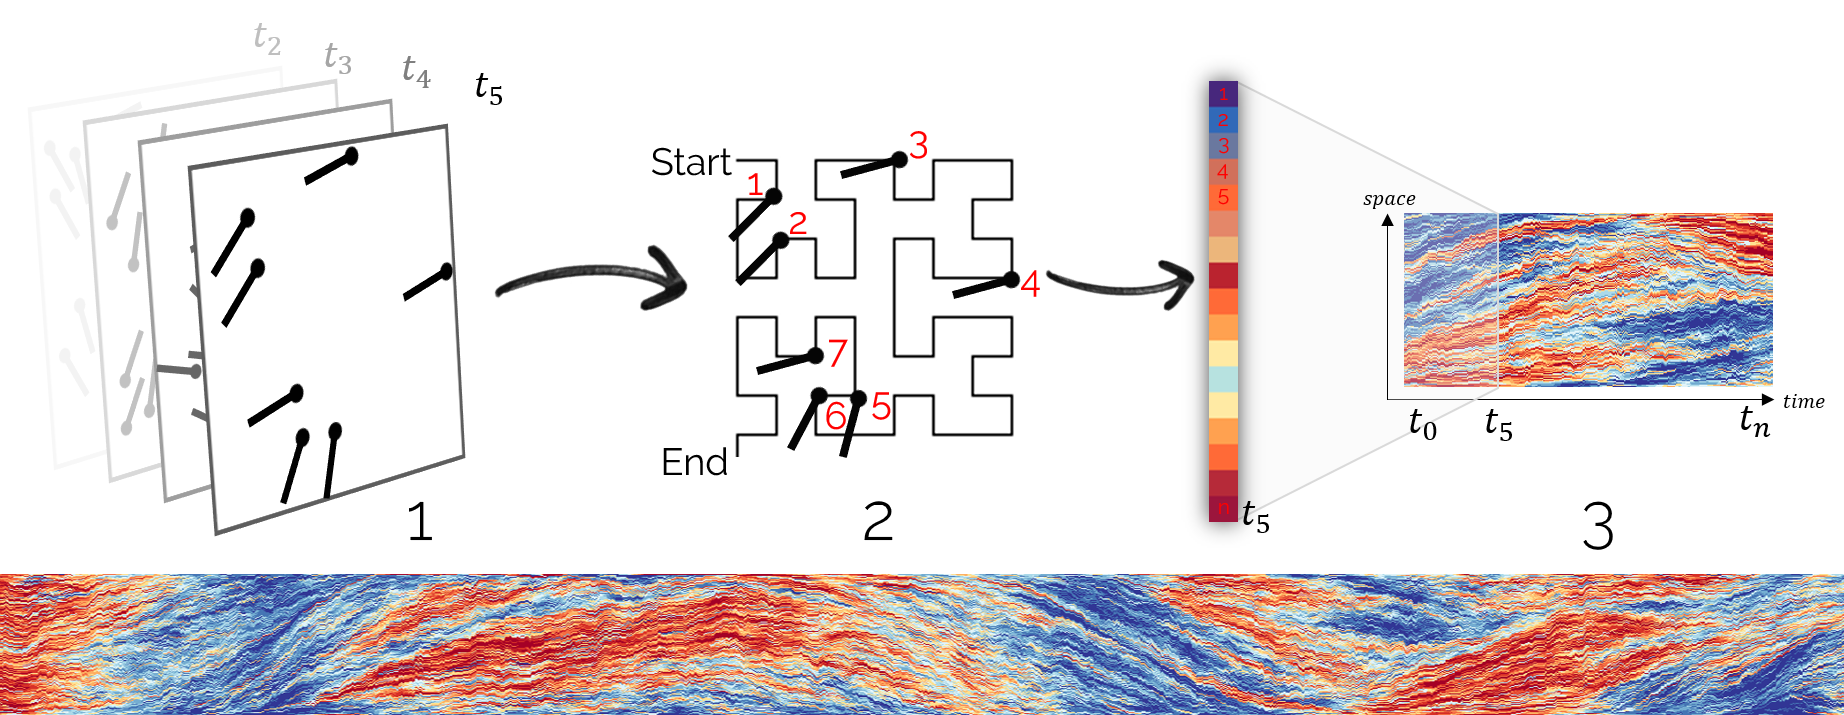
\includegraphics[width = \textwidth]{src/imgs/motionrugs.png}
    \caption{Source: \cite{Buchmuller:2018:MVCTST}. Pipeline of the MotionRugs visualization technique, the data used is the movement of a set of fish in an aquarium.}
    \label{fig:motionrugs}
\end{figure}

In Fig.~\ref{fig:motionrugs} is presented an example of the method MotionRugs and the process of generating the visualization.
%
Each time frame is represented as a column, the column is filled with pixels, one for each object in the space, that are ordered based on a projection method.
%
In the example, it is a visualization generated from a set of fish moving in circles in an aquarium, each pixel in the column is a fish. 
%
The beautiful result of the visualization is obtained with the coloring based on the velocity of each fish.
%
With this view, it is possible to observe the general movement of observed entities, comparing different timestamps without occlusion or distortions.

%
As the objective of the method is to visualize collective moments, it only considers the relative position between objects and only permits the interpretation of the group trend of movement.
%
Besides that, it is limited to trajectories of objects that are observed in the complete period, so in the scenario of spatio-temporal events with small periods of occurrence, there is not a simple adaptation.
